\chapter{Algoritmi greedy}
\section{Introduzione e definizione}
Gli \textbf{algoritmi greedy} (golosi), sono una classe di algoritmi che prende sempre una
soluzione ottima localmente, nella speranza che tale soluzione porterà ad una
ottimalità globale. Infatti questo tipo di algoritmo non funziona sempre, ma se 
riusciamo ad usarlo è preferibile per motivi di semplicità ed efficienza. Vediamo degli esempi:\smallskip\\
Abbiamo già visto nel capitolo precedente (\ref{Coin Change Analysis}) il problema del \textit{Coin Change Analysis}.
Questo problema è un esempio perfetto per capire che un approccio \textbf{greedy} può funzionare
(rendendo il problema nettamente più semplice ed efficiente), o non funzionare.\\
Infatti avevamo visto che se il sistema monetario non è canonico (canonico vuol dire che l’uso del taglio massimo fa
sempre parte della soluzione), non era possibile utilizzare un algoritmo greedy, ma dovevamo utilizzare
la programmazione dinamica che rendeva l'algoritmo molto più dispendioso e complesso.\\
Se invece il sistema monetario è canonico, possiamo utilizzare un approccio greedy,
prendendo sempre il taglio di moneta più grande disponibile fino a raggiungere il
target (vd \ref{Coin Change Analysis}).\smallskip\\
La \textbf{strategia} che caratterizza un algoritmo greedy è:
\begin{itemize}
    \item Si valutano l'insieme di opzioni disponibili.
    \item Si sceglie quella che sembra migliore nel breve termine (la scelta "greedy"),
    che porterà ad un ottimo locale.
    \item Si procede senza ripensare alle decisioni fatte (che è esattamente il contrario
    di quello che si fa con la programmazione dinamica).
\end{itemize}
Un problema si può affrontare con un approccio greedy se possiede queste due caratteristiche:
\begin{itemize}
    \item \textbf{Greedy choice property}: una scelta locale ottimale porta ad una soluzione
    globale ottimale.
    \item \textbf{Optimal substructure}: la soluzione ottimale del problema contiene le soluzioni
    ottimali ai suoi sottoproblemi.
\end{itemize}
Nelle prossime sezioni vedremo problemi risolti con degli algoritmi greedy.



\section{Problema della codifica di Huffman}
Dato $S = \{ s_1, s_2,\dots ,s_n\}$ un insieme di $n$ caratteri e che ogni carattere
$c \in C$ sia presente con una certa frequenza $f_i$. L'\textbf{obiettivo}
è:
\begin{enumerate}
    \item Assegnare ad ogni simbolo un codice binario (0 o 1), creando un prefisso (detto \textit{codice di Huffman}) che
    identificherà univocamente il simbolo.
    \item Minimizzare la lunghezza della media pesata $\left(  \sum^{i} f_i \times l_i
    (\text{lunghezza codice di } s_i)  \right)$ 
\end{enumerate}
Visto che a parole può risultare poco chiaro, vediamo un esempio e successivamente spieghiamo
la strategia di risoluzione.

\begin{figure}[H]
    \centering  
    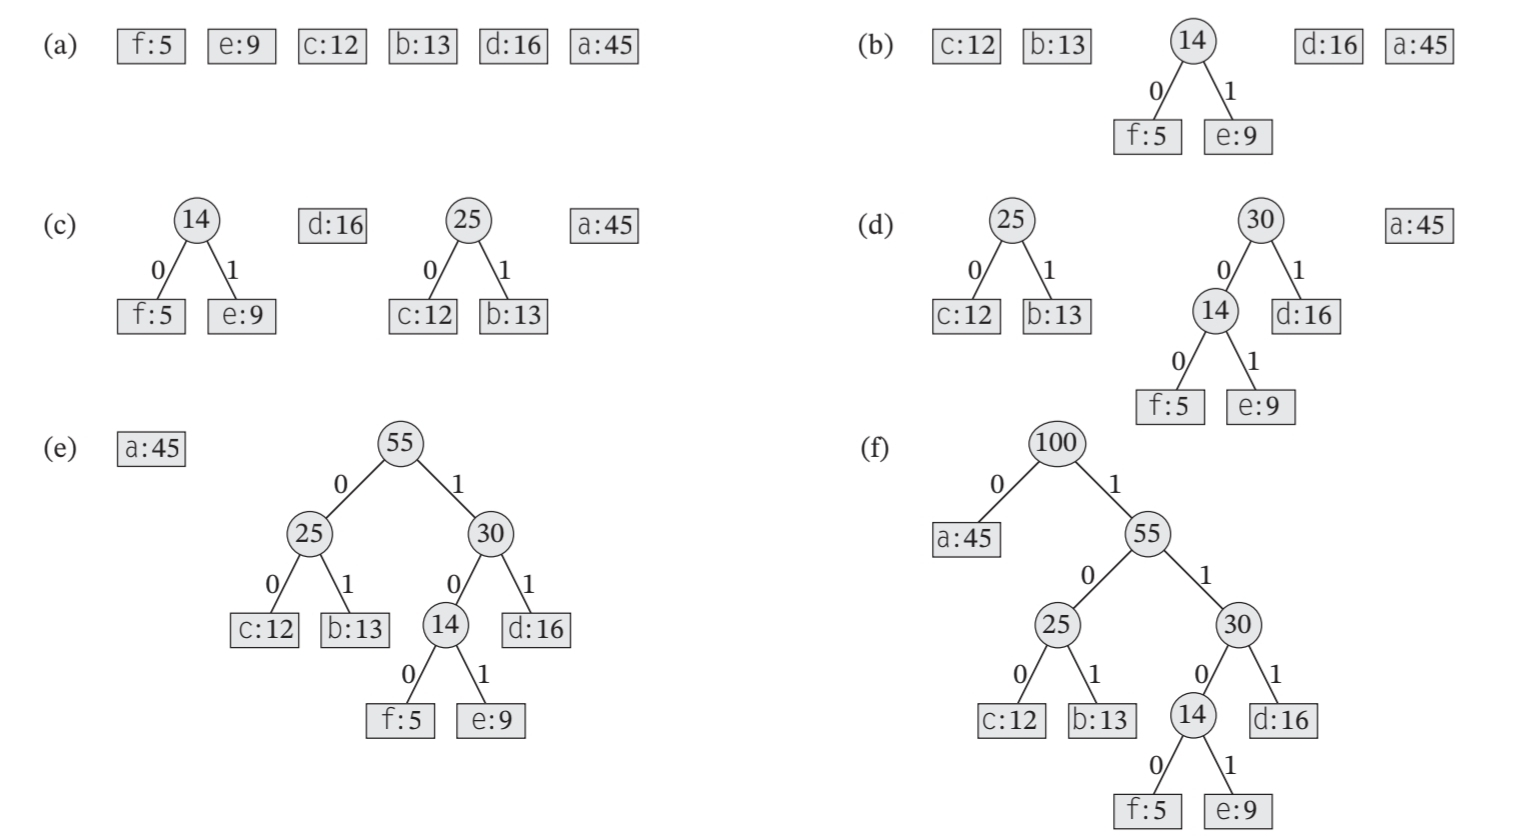
\includegraphics[width=1\linewidth]{../images/esempio_Huffman.jpg}
\end{figure}
\noindent Questi sono i passi dell'algoritmo di Huffman $\Big( (a) \rightarrow (b) \cdots \rightarrow (f)  \Big)$, la \textbf{strategia} è la seguente:\\
All'inizio abbiamo i dati di input, ovvero i caratteri con la rispettiva frequenza. 
Consideriamo ogni dato come radice di un albero binario. A ogni passo i due alberi 
con le frequenze più piccole vengono fusi, quindi questi due alberi diventano figli di un nuovo nodo 
rappresentante la somma delle frequenze degli alberi che sono stati fusi. Ad ogni fusione
vengono assegnati i codici binari, in questo caso la regola è: un arco che collega un nodo interno con i suoi figli
ha l'etichetta 0 se è un arco che congiunge il figlio sinistro, ha l'etichetta 1 se è un arco che congiunge 
un figlio destro.\\
Ripetendo questo procedimento fino ad ottenere un unico albero binario abbiamo ottenuto che ogni carattere ha 
il proprio codice che lo rappresenta, formato dalla sequenza di codici binari (0 o 1) a partire dalla radice 
dell'albero completo fino alla foglia che rappresenta il carattere. In questo esempio guardando l'ultimo step $(f)$, si ha che:
\begin{itemize}
    \item \textbf{f:5} $\to 1100$
    \item \textbf{e:9} $\to 1101$
    \item \textbf{c:12} $\to 100$
    \item \textbf{b:13} $\to 101$
    \item \textbf{d:16} $\to 111$
    \item \textbf{a:45} $\to 0$ 
\end{itemize}
Il codice per creare questo albero è:
\begin{verbatim}
    while (heap->size > 1) {
        left = extractMin(heap);
        right = extractMin(heap);
        top = createNode('$', left->freq+right->freq);
        top->left = left;
        top->right = right;
        insertMinHeap(heap, top);
    }
\end{verbatim}

\noindent Come è ben visibile dall'esempio, i simboli con le frequenze minime $f_i$ 
si trovano alla massima profondità dell'albero. Visto che la \textbf{lunghezza media pesata} 
è calcolata come $\sum^i (f_i \times l_i)$, e che più la frequenza è alta, minore è il 
codice binario associato al carattere che ha tale frequenza, la lunghezza media è \textbf{minima}.






\section{Problema di Activity selection}
Il problema della selezione di attività consente di selezionare il più grande
insieme di attività compatibili. Più formalmente diciamo che:\\
Dato $A = \{ a_1, a_2,\dots, a_n \}$ un insieme di attività, dove ciascuna attività $a_i$
ha un tempo di inizio $s_i\in \mathbb{R}$ e un tempo di fine $f_i\in\mathbb{R}$
con $s_i< f_i$, e dato il vincolo di compatibilità: $a_i$ e $a_j$ sono compatibili se non si sovrappongono nel tempo
$\left([s_i,f_i]  \cap [s_j,f_j]  = \emptyset     \right)$, l'\textbf{obiettivo} di trovare un sottoinsieme $A' \subseteq A$ tale che:
\begin{itemize}
    \item Tutte le attività in $A'$ sono compatibili.
    \item $|A'|$ è il massimo possibile, ovvero il numero di attività del sottoinsieme soluzione è massimo.
\end{itemize}
La \textbf{strategia} per risolvere questo problema con un approccio greedy è la seguente:
\begin{enumerate}
    \item Ordina le attività di $A$ per tempo di fine crescente, ovvero $f_1 \le f_2 \le \cdots \le f_n$.
    \item Inizializza $G \leftarrow \emptyset$ e $t = 0$, dove $G = \{ g_1,g_2,\dots,g_k  \}$ è l'insieme delle attività selezionate dall'algortimo greedy, all'inizio ovviamente
    sarà inizializzato come un insieme vuoto.
    \item Realizza il ciclo che ad ogni iterazione aggiorna le varibili sotto certe condizioni, ovvero se $s_i \ge t$ aggiungo $a_i$ a $G$ e pongo $t \leftarrow f_i$, in
    questo modo scarto le attività che si sovrappongono e in $G$ andranno solo quelle che rispettano il vincolo di compatibilità.
    \item Restituisce $G$
\end{enumerate}

\noindent Il codice quindi sarà (supponendo che gli eventi in $A$ siano già ordinati):
\begin{verbatim}
    GREEDY-ACTIVITY-SELECTOR(s, f, n, A) {
        G = {};
        t = 0;
        for i = 1 to n
            if s[i] >= t
                G.add(A[i]);
                t = f[i];
        return G;
    }   
\end{verbatim}

\subsection{Dimostrazione dell'ottimalità}
Vogliamo dimostrare che l'approccio greedy ci dà effettivamente un risultato ottimale. Sia $G = \{  g_1,g_2, \dots , g_k  \}$ l'insieme 
delle attività selezionate dall'algoritmo greedy, sia $O=\{  o_1,o_2,\dots, o_m   \}$ un sottoinsieme ottimo, cioè un insieme di attività compatibili
con $m\ge k$. L\textbf{obiettivo} è dimostrare che $\bm{k = m}$, cioè che l'algoritmo greedy seleziona tante attività quante ne ha 
una soluzione ottima. Procediamo per \textbf{induzione}:\smallskip\\
Costruiamo un altro insieme $O'$ tale che tutte le sue attività sono compatibili
(non si sovrappongono le attività) e che $|O| = |O'|$ (soluzione ottima).
\begin{itemize}
    \item \textbf{Passo base}:
    \begin{itemize}
        \item confrontiamo $g_1$ con $o_1$, e avremo che $f_{g_1} \le f_{o_1}$ per costruzione, poichè in $G$ ci sono
        le attività scelte dall'algoritmo Greedy, il quale sceglie le attività che finiscono prima.
        \item sostituiamo $o_1$ con $g_1$ in $O$
        \item dopo la sostituzione otteniamo un insieme $O'$ che ha tutti gli elementi di $O$, ma con
        la prima attività che è diventata $g_1$, ovvero $O' = \{ g_1, o_2, o_3, \dots, o_m  \}$.
        \item Notiamo che l'insieme $O'$ è ancora ottimo, perchè l'attività $g_1$ che abbiamo inserito è compatibile
        con tutte le altre attività dentro $O'$, visto che finisce prima.
    \end{itemize}

    \item \textbf{Passo induttivo}
    \begin{itemize}
        \item supponiamo di aver già sostituito le prime $r$ attività in $O$ cone le prime $r$ in $G$,
        ottenendo un insieme $O'$ ancora ottimo, dobbiamo mostrare che possiamo sostituire anche $g_{r+1}$ a $o_{r+1}$, 
        mantenendo una soluzione ottima.
        \item $o_{r+1}$ essendo compatibile con $g_r$, deve iniziare dopo $f_{g_r}$, l'algoritmo greedy sceglie
        l'attività che finisce prima, quindi sceglie $g_{r+1}$. 
        \item sotituiamo anche $o_{r+1}$ con $g_{r+1}$, siccome $f_{g_{r+1}} \le f_{o_{r+1}}$.
    \end{itemize}
\end{itemize}
Alla fine di tutti i confronti abbiamo che $O' = G$, che è la soluzione ottima scelta dall'algoritmo greedy. 
In questo procedimento non abbiamo scartato alcuna attività, ma abbiamo solo sostituito facendo rimanere la soluzione ottima,
quindi abbiamo dimostrato che $\bm{k = m}$.



\section{Confronto con altri approcci}
\begin{table}[ht]
    \centering
    % Aggiunge un po' di spazio in altezza alle celle per non farle sembrare schiacciate
    \renewcommand{\arraystretch}{1.3} 
    
    % La prima colonna ha una larghezza fissa di 3.2cm, le altre 3 si dividono lo spazio rimanente (X)
    \begin{tabularx}{\textwidth}{|p{3.2cm}|X|X|X|}
        \hline
        
        % Sfondo verde scuro per la prima riga
        \rowcolor{SALZO} 
        
        \multicolumn{1}{|c|}{\textbf{caratteristica}} & 
        \multicolumn{1}{c|}{\textbf{greedy}} & 
        \multicolumn{1}{c|}{\textbf{programmazione dinamica}} & 
        \multicolumn{1}{c|}{\textbf{divide et impera}} \\ 
        \hline
        
        \textbf{strategia principale} & 
        scelte locali ottimali & 
        risoluzione e memorizzazione di sottoproblemi & 
        divisione in sottoproblemi indipendenti \\ 
        \hline
        
        \textbf{approccio} & 
        iterativo & 
        iterativo o ricorsivo con memoization & 
        ricorsivo \\ 
        \hline
        
        \textbf{ottimalità} & 
        solo se problema ha proprietà greedy & 
        sempre (se struttura ottimale esiste) & 
        non garantita direttamente \\ 
        \hline
        
        \textbf{dipendenza tra sottoproblemi} & 
        non considera sottoproblemi & 
        i sottoproblemi si sovrappongono & 
        i sottoproblemi sono indipendenti \\ 
        \hline
        
        \textbf{efficienza} & 
        molto veloce ($O(n)$ spesso) & 
        più lento ($O(n^2)$ o $O(n^3)$ tipico) & 
        dipende dalla profondità della ricorsione \\ 
        \hline
        
        \textbf{uso della memoria} & 
        basso & 
        alto (per salvare soluzioni parziali) & 
        variabile \\ 
        \hline
        
        \textbf{esempi classici} & 
        cammini minimi (Dijkstra), Kruskal & 
        Zaino 0/1, Fibonacci, allineamento di sequenze & 
        MergeSort, QuickSort, Ricerca binaria \\ 
        \hline
        
        \textbf{punti di forza} & 
        semplicità, velocità & 
        precisione, correttezza garantita & 
        suddivisione naturale di problemi complessi \\ 
        \hline
        
        \textbf{punti deboli} & 
        rischio di soluzioni subottimali & 
        maggior consumo di tempo e memoria & 
        richiede problemi naturalmente divisibili \\ 
        \hline
        
    \end{tabularx}
\end{table}